\documentclass[11pt]{report}
\usepackage{fullpage}
\usepackage{graphicx}
\usepackage{float}
\restylefloat{table}
\begin{document}

\title{Autism Simulator}
\author{Ashley Peacock}
\maketitle
\tableofcontents

\chapter{Introduction}
For this report I will be giving the overview of my thesis thus far which includes work carried out this semester and some incomplete sections (with notes as to what will be in there or improvements)

\section{Selecting a project}
The project started with the purpose of creating software to benefit someone with autism or ADHD or those in contact with these conditions such as family members or carers. Owing this is a very broad topic it was important to create multiple proposals and select the most useful. All proposals were put on a website and a selection was made after considering results from an online survey, conversing with professionals and people with ASD and considering systems and research currently available.

Project proposals:
\begin{table}[H]
    \begin{tabular}{| p{4cm} | p{9cm} |}
    \hline
    Proposal name & Description                                                                  \\
    \hline
    \hline
    Online diary & Online system to improve communication between carers, parents, social workers, schools. Parties could post questions and ask for suggestions when dealing with certain behaviours as well as document the child's day allowing easier identification of patterns of behaviour or problems                    \\
    \hline
    Social simulator & Simulated social scenarios for autistic users to trial various social situations and see possible outcomes  \\
    \hline
    Dynamic scheduler and planner app & A planner that would re-schedule tasks when not completed and present basic to-do lists with tasks broken down into manageable chunks  \\
    \hline
    Environment app & Phone app aimed to encourage children to look and question their environment \\
    \hline
   Autism simulator & A 3D virtual environment where the user plays as a child with autism and can thus experience some of the obstacles faced through a visual/game environment \\
    \hline
    \end{tabular}
\end{table}

\subsection{Questionnaire}
A questionnaire was anonymously completed by six people in total and included people with ASD/ADHD, professionals, carers and parents and was compiled with both qualitative and quantitative questions.

\begin{enumerate}
\item Please give some information about yourself, for example if you have ASD/ADHD or are a professional/carer.
\item Please select and rank three proposals you feel are the best
\item Please explain reasons for selection
\end{enumerate}

\subsubsection{Results}

Below summarises some of the comments given in the feedback questionnaire as well as considerating factors from other areas

\begin{table}[H]
    \begin{tabular}{| p{4cm} | p{8cm} |}
    \hline
    Proposal name & General reasons for/against                                                                 \\
    \hline
    \hline
    Online diary & For: Cross communication between doctors, teachers, parents and carers which is often problematic with information missed. Against: Good in theory but may not be practical due to data protection. Relies too heavily on parents/carers being able to read emails or notifications. May be difficult for some schools to gain access to wifi.                \\
    \hline
    Social simulator & Against: Big project given the time-frame. Other companies working on a similar concept. Much research on this topic already. Conveying 'social stories' could be a better approach to deal with context specific situations. \\
    \hline
    Dynamic scheduler and planner app & Against: least unique proposal, many other planners available. For: No planners available that specifically target planning/executive functioning difficulties within ADHD and Autism \\
    \hline
    Environment app & Against: Hard to back with literature. Difficult concept to understand(possibly not explained well) For: Least amount of implementation work. Could be simply but effective. \\
    \hline
   Autism simulator & Against: Big project given the time frame, no previous simulators which can be drawn from. For: Most unique and popular idea. Misunderstanding from the general public is a big problem. Could be extremely helpful for teacher's training. \\
    \hline
    \end{tabular}
\end{table}

** TODO: Give more quotes and information from questionnaire from people who gave feedback.

\subsection{Choice}

In summary, the selection of the project followed by considering:

\begin{enumerate}
\item Advantages and disadvantages of all options.
\item Looking at factors such as time constraints and the learning curve involved for each.
\item Conducting an online survey.
\item Speaking to a range of individuals at the ADDISS ADHD conference(London 2012) which also contained parents and professionals with experience and knowledge of autism.
\end{enumerate}

From all sources it became evident that the autism simulator was the most unique and useful concept with the only concern being its potential size and lack of restriction. This was the final project chosen as it was felt
if focus was directed onto conveying just the sensory differences within autism to start with and a game engine was selected rather than developing from scratch, it would be attainable in the given time-frame.

\chapter{Literature review}

\section{What is Autism?}

Autism is a life-long condition which affects how an individual may perceive and communicate to the world around\cite{nas}. It is currently diagnosed by the presence of atypicalities in three domains(collectively known as the triad of impairments): social imagination, social communication, social interaction. In addition to these are non-diagnostic but highly prevalent features such as sensory abnormalities, information processing difficulties and prosopagnosia\cite{blah}. 

As a spectrum disorder, the range and severity of symptoms are completely unique to each person and as such it can be quite difficult to diagnose. For those unaware of the condition and the more hidden aspects, it can be difficult to accept as a genuine problem for parents to seek support or sympathies from the public for behaviours such as meltdowns which appear like tantrums.

For those with autism on the high-functioning side of the spectrum(i.e Aspergers) their difficulties can be less obvious; they may develop superb language skills but have difficulty using these in a social context, leading to unintentional social offence or ridicule. Difficulties with social imagination and theory of mind can make it difficult to see another person perspective and thus understanding why they have been perceived in a way far from their intentions is made challenging. In contrast, those on the low-functioning side of the spectrum may have little to no verbal language and prefer to communicate using visual mediums such as PECS. 

With some of the disadvantages that may come with having autism, there are reported strengths as a result of having a unique cognitive style for example a talent for spotting details\cite{bayes} or having an impeccable memory of facts in relation to their 'special interests'. 

Public perceptions of autism as discussed later in more detail greatly differs. Aspergers syndrome has only been included in the DMV since 1991 and as later seen from interviews of those with late diagnosis, it was still hard for their own parents to accept it as a condition and tangible explanation and not simply an excuse for "bad behaviour". In the last decade there has appeared to be improvements in public perception and understanding of autism and other cognitive differences such as dyslexia and adhd, but there is still much left to be desired. 

- add a bit of information/brief introduction on repetitive behaviours


\section{Triad of Impairments}

**** This section needs to be re-written once I can find DSM-V changes. \\

There are three key areas of difficulty that people with autism share.

\subsubsection*{Social communication}
People with autism have difficulty with verbal and non-verbal language such as body language or tone of voice. Language tends to be interpreted literally and thus metaphors, sarcasm and jokes can be difficult to understand\cite{nas}. An example of literal interpretation is where a person with autism misunderstood the question "What's up?" and proceeded to look up at the ceiling. Other communication difficulties include echolalic language(repeating language said to them) or speaking excessively about their 'Special interests' without detecting that the other party may be bored\cite{nas}. Although people with autism will usually understand what is being said to them they may prefer to use visual symbols such as PECS(Picture Exchange Communication System). 

Due to literal language interpretation, it is important that language communicated is clear, concise and unambiguous, one of the needs the public were most unaware of\cite{autismmisconception}.

\begin{quote}
Most things I take at face value, without judgement or interpreting them. I look at them in a concrete, literal and very individual way. \cite{olgab}
\end{quote}

\subsubsection*{Social interaction}

\begin{quote}
Autistic people have to understand scientifically what non-autistic people already understand instinctively 
- Mark Segar, Autistic Survival Guide.
\end{quote}

Many people with autism have difficulty giving eye contact, one person described eye contact as "physically painful". By not giving eye contact, it may cause social queues such as facial expressions to be missed, potentially leading to inappropriate responses. Lack of eye contact could be perceived as rude or not paying attention to the speaker, causing possible unintentional offence. Other social interaction difficulties reported include trouble understanding social rules\cite{nas}, for example why people say 'thankyou'.

\subsubsection*{Social imagination}
Social imagination deficits result in difficulties 'Putting themselves in another person's shoes', also known as 'Theory of mind'. Other resulting difficulties include problems predicting events or identifying possible dangers such as running across a road and consequently, new situations can be difficult.\cite{nas}

Social imagination difficulties can make it hard for a child with autism to engage in imaginative play, preferring to act out scenes from films identically which can make it difficult for other children interacting with them if they prefer to deviate or explore a new plot.\cite{nas}

\section{Information processing}

It is suggested that people with autism process information holistically, a theory known as Gestalt perception. Gestalt perception is posited to be a cause of fragmented or distorted perceptions in people with autism\cite{olgab}; processing information as a whole instead of in parts make it difficult to drawn connections and thus make predictions about the world. "I had always known that the world was fragmented. My mother was a small and a texture, my father was a tone, and my older brother was something, which was moving about" \cite{williams1992}. 

It is argued that people with autism perceive the world more accurately because their inferences are less dependent on previous experience but a negative consequence of this is being less able to filter irrelevant stimulus \cite{bayes}. Difficulties filtering information can cause problems differentiating between background and foreground noise and so in a room with many people talking it may be hard to tune into an individual conversation \cite{bayes}. 

Delays in information processing are a common feature in autism. In extreme cases, it can take weeks, months or even years to process information and one of the reasons given to the cause lye in the theory of gestalt perception. Processing information as a whole leads to over-selectivity and thus even familiar environments are looked upon as entirely new and one small change to the environment can cause a large amount of distress\cite{olgab}. This would offer a suggestion as to why people with autism have a strong desire for strict routine. Questions asked to a person with autism should be given ample time for a response, if their process of thought is interrupted it can cause a complete disruption and the individual has to start this process again\cite{olgab}. As a result of distorted perception, it may take someone with autism longer to adjust to their surroundings. 

Distortions are reported to become worse in the state of nervous over-arousal and information overloads\cite{olgab} and thus a cycle of problems occurs; the more stressed a person with autism may be, the more these distortions occur and the harder it is to make sense of the world, consequently resulting in even more stress.

\subsection{Sensory processing}

While social and communication difficulties are core symptoms and most commonly associated with autism in the public view, "Many people with Asperger syndrome/High functioning autism define their sensory processing problems as more disabling than the deficits in communication/social behaviour\cite{olgab}. Sensory processing differences in autism are highly reported, 81\% of respondents reported differences in visual perception, 87\% in hearing, 77\% in tactile perception, 30\% in taste and 56\% in smell \cite{sensory_leisure}. Senses play a vital role in how we model and perceive the world around us so if one senses the world in a differently, their view and resulting behaviours will also be different. 

Senses in autism can be hyper(more sensitive), hypo(less sensitive), agnostic or fluctuate between hyper and hypo\cite{bayes}. As with all areas of autism, sensory atypicalities differ and are unique to each individual, however, these fluctuations make it an area of particular challenge for carers and for a person with autism to identify or predict troubling sources before they occur. Fluctuations can be described as a 'FM radio that is not exactly tuned on the station when you are driving down the freeway. Sometimes the world comes in clearly and at other times it does not" \cite{olgab}.

When a sensory channel is in a state of agnosia, although able to see, one may not be able to assign it to any meaning. The result is one can become 'mind-blind', or 'mind-deaf' where the person can appear as if they are genuinely deaf.

Catering with for the many different sensory needs for many different children can be very demanding. In the classroom if a child is hypo-visual and feels a need to stimulate their visual senses by constantly switching on and off a light, in contrast to another child in the class being hyper sensitive, the result could lead to a sensory or information overload(this was commented on in one of the interviews from the teacher...).

Below are some examples of the effects someone with autism may experience depending on the state of their sensory channel:

\begin{table}
    \begin{tabular}{| l | p{5cm} | p{5cm} |}
    \hline
    Sense channel & Hyper                                                                                                                      & Hypo                                                                   \\
    \hline
    \hline
    Vision        & Vision may be magnified                                                                                                    & Attracted to light or fascinated with bright colors                    \\
    \hline
    Auditory      & Sounds are amplified. Temple Grandin a write with autism described her ears as like 'microphones'                          & Is attracted to sounds/noises                                          \\
    \hline
    Tactile       & Clothes may hurt. One person with autism described clothe labels as feeling like 'barbed wire'. May not like being hugged. & Enjoys being hugged or seeks pressure by crawling under heavy objects. \\
    \hline
    Taste/Smells & Smells or texture of foods may be intolerable. & Mouths and licks objects \\
    \hline
    Vestibular & Difficulty with walking or crawling on uneven or unstable surfaces. & Spins, runs round and round, rocks back and forth \\
    \hline
    \end{tabular}
\end{table}

// (below is probably not much use at the moment, but useful for later justifying the game character's traits and responses to the environment if I can structure it in properly...)

Sensory processing patterns can be categorised into four-types\cite{sensory_leisure}:

\begin{enumerate}
\item Sensory avoidance pattern: Low sensory threshold. 
\item Sensory seeking patterns: A high sensory threshold and make seek out stimulus.
\item Sensory sensitivity patterns: Low thresholds and may respond to stimulus more intensely or for a longer period of time.
\item Low registration: High sensory threshold, may appear not to detect incoming sensory information and also show a lack of responsiveness.
\end{enumerate}

Correlation between sensory difficulties and difficult temperament characteristics such as activity level, adaptability to changing context, quality of mood, threshold of responsiveness, intensity of reaction and persistence\cite{temperament}. 

\subsection{Sensory and Information overload}

*** Need more comments and to hunt down literature which I have definitely read somewhere which explains more of what it is actually like to experience a sensory overload. Justification for lights becoming brighter is below. \\

When the amount of information required to be processed comes in large volumes too quickly it can result in an 'Information' or 'Sensory' overload. Overloads can result in hypersensitivity causing lights becoming brighter or sounds becoming louder. Visual/auditory causes of overloads can cause tactile sensitivity and so being touched might become painful. Donna Williams reports that "sensory overload caused by bright lights, fluorescent lights, colours, and patterns makes the body react as if being attacked or bombarded, resulting in such physical symptoms as headaches, anxiety, panic attacks or aggression"\cite{bayes}.

The resulting behaviours again differ for each individual and are discussed in the following section.

\subsection{Resulting behaviours}


\subsubsection{Meltdowns}
If a sensory overload is not dispersed quickly enough it can lead to a full sensory shut-down in which all senses enter a state of agnosia and the person with autism withdraws from the world. Another reaction to a sensory overload is entering a state of 'fight or flight', running away from the source without any sense of danger, or exhibiting temper-like tantrums or self injurious behaviour. These behaviours can be collectively known as 'meltdowns'; the individual experiencing them feels a loss of control. Meltdowns can be caused by not only by sensory, but an emotional and cognitive overload.

\subsubsection{Mono-processing}
Mono-processing is described as an involuntary response to information overloads where all but a few sensory channels are closed. Vision may become hyper-sensitive whilst but the individual may not be able consciously hear. Subconsciously however, this information may be absorbed and processed later, further increasing the information processing delay. 


\subsubsection{Repetitive and restricted behaviours}

// Note: find information on 'attractive stimulus' and Sensory soothing objects. Relate it more to content that can be use as justification for simulator choices.

Repetitive and restrictive behaviours are highly prevalent in people with autism and are thought to be caused by:
\begin{enumerate}
\item Needing to induce sensory sensory stimulation\cite{rrsyouth}.
\item As a reaction to sensory stimulation\cite{rrsyouth}.
\end{enumerate}

Repetitive behaviours and sensory issues have been found to be positive correlated\cite{rrs_sensory}\cite{rssyouth}. High levels of restricted behaviours were associated with less severe levels of depression, indicating that such behaviours may act as a mechanism to protect against or be a direct cause\cite{rss_ensory}. Those with low-functioning autism were more likely to engage in repetitive behaviours such as 'stimming', repetitive manipulation of objects and self-injurious behaviour in contrast to high-functioning autism having restricted interests, language or attachment to objects\cite{rss_sensory}. People with high-functioning autism were reported to have higher levels of anxiety with restrictive behaviours thought to a developed coping mechanism\cite{rssyouth}.

93\% of children with autism were reported to be distressed by change \cite{fears}. With an ever changing perceptions of the environment, routine can be their only sense of familiarity and reassurance. Interestingly it is reported that people with autism can have more problems with small changes in a familiar environment in comparison to entirely new situations\cite{bayes}.  

\section{Effect of Autism}

Social interactions are unpredictable following no set guidelines or rules and differing from culture to culture. For one to feel part of a group we need positive reinforcement that our actions fit within that group. Continuity helps us build feelings of safety and security which can be transferred to social trust, allowing us to predict the behaviours of people around us and reduce uncertainty. For many of us, we take for granted our innate ability to know when and how to communicate, but for someone with autism they have to learn scientifically what we have learnt naturally. Receiving negative feedback in social encounters can result in feelings of embarrassment or ridicule, threatening an individuals ontological security which has further possible consequences; a negative self-image, the world and future.

It is proposed that it is our moral duty to be compassionate and sympathetic towards the group, to monitor our facial expressions and reactions as to not cause offence. This can be problematic in two ways - if the group have little understanding of someone who is different the group cannot adjust to the individual. Likewise if the individual struggles to understand the workings of the group, they cannot adjust and consequently feel an outcast. 

One person with Aspergers syndrome(a form of high-functioning autism) it as like "living in a bubble or living on the other side of a plate glass window to everybody else. It is like you are just a spectator in this thing"\cite{aspieway}. In interviews conducted by Sara Ryan and Ulla Raisanen(2008) three themes emerged: not belonging, trying to fit in and the need for safe spaces. Inspite of this, interviews showed their desire was not to rid themselves of Aspergers but to simply fit into main-stream society. Interviewees were extremely aware of their differences but inspite of desperately trying to learn the rules and social norms it was often felt their efforts were not reciprocated by neurotypical people.

Of course, one solution to aid those on the Autistic spectrum to fit into main-stream society would be increase public awareness, acceptance and understanding. However, explaining emotions and feelings has proven to be extremely challenging for some individuals which makes such possibilities difficult to achieve. The act of trying to express themselves with words was described as painful \cite{aspieway}. 

\subsection{Effects on children with ASD}

Notes on things supervisor has suggested writing here:

State what difficulties from what part of the spectrum and age group. At the moment using examples and symptoms from the higher end of the spectrum when it should be more for young children/lower part of the spectrum. Social communication difficulties would therefore be more like eye-contact, responding to cues such as name being called and any use of language. Language delays are a huge feature of pre-school children with autism.\\
Social interaction - emphasize child-level issues i.e taking turns, sharing enjoyment with others.\\
Social imagination - Emphasize interests and repetitive behaviours here. I.e lining things up, limited play such as playing with parts of objects, obsessive fixations on specific toys and specific routines\\

\subsubsection{Unusual fears}
It was found that 40\% of children with autism had unusual fears in comparison to 0-5\% of typical children, the vast majority of these were made up of mechanical objects. Children with autism have higher levels of anxiety than typical children\cite{fears} and increased anxiety from being faced with more fears on a day to day basis will only increase this and further impact on functioning. For example, not leaving the house because it's cloudy, or not taking a shower because of the noise from the drain, not going to school due to being afraid the fire alarm will sound. The top five reported unusual fears were toilets, elevators, vacuum cleaners, thunderstorms, tornadoes. The cause of many of these unusual fears in children with autism are thought to be related to sensory perception differences\cite{fears}.

\subsection{Effects on families}
- this probably links into public perception but might be able to find some interesting and relevant material here...

\section{Impact and Prevalence}
Figures drawn from the 2011 census estimate that 1.1\% of the population have Autism\cite{nas}. This figure appears to be rising across the globe as awareness and understanding of the condition increases alongside broadening criteria\cite{increasingprevalence}, Aspergers syndrome is one example addition and which has only been a formal diagnosis since 1990. Early counts of people with autism spectrum conditions were less than 10 in 10,000, this has grown to a new prediction of 110 in 10,000 in the USA \cite{increasingprevalence}.

It is estimated that only 22\% of teachers have been trained specifically in autism and the majority of training given is typically one to four hours. 54\% of all teachers in England do not feel they have had adequate training to teach children with autism.\cite{statsandfacts} 30\% of parents of children with autism in mainstream education are satisfied with the level of understanding of autism across the school\cite{nasschool}. 23\% of parents are dissatisfied with SENCO's level of understanding of autism. 

Figures obtained show that approximately 40\% of children with autism have been bullied at school. 1 in 5 children with autism have been excluded from school \cite{nasschool} and only 24.4\% of pupils with autism achieved 5A*-C GCSEs in 2010/2011 in comparison to 58.2\% of the overall population\cite{statsandfacts}, a surprising figure owing people with autism are deemed to have above average intelligence, indicating difficulties at school may be a reason for not for-filling potential. 

\begin{quote}
Danny would not have been excluded if the school had understood the difference between 'normal' behaviour and Aspergers syndrome. They inflamed situations because they didn't understand that my son finds physical contact, or being touched by teachers, really difficult \cite{nasschool}
\end{quote}

\begin{quote}
If I could make one change...I would ensure compulsory, thorough training about autism and how it affects learning is given to all school staff. \cite{nasschool}
\end{quote}

\section{Public perception}
Although there is some level of awareness of autism in the public domain, there is still much left to be desired.  A survey carried out by the National Autistic Society showed that 92\% of respondents had heard of Autism but only 48\% had heard of Aspergers syndrome which has less obvious difficulties. Most were able to identify key characteristics of autism such as difficulty communicating or making friends. Other common characteristics such as a need for 'clear unambiguous instructions' and sensory hypersensitivity were less known\cite{autismmisconception}. 

\begin{quote}
If I could make one change... every person who comes into contact with my daughter would have some form of training in autism.\cite{nasschool}
\end{quote}

\section{Previous work}

\subsection{Education software}
How other education software can be used to help children with understanding autism or general learning. Include information from the paper Alyssa sent.

\subsection{Other Autism simulations}

In Febrary 2013 a playable 3D virtual environment depicting sensory difficulties in autism was released. The simulation allowed the user to navigate around a playground with other children who are all identical and if the user gets too close to them, visual distortions occur and high-pitched sounds are played. The simulator from the public perspective was very well received and thought as a good step in increasing awareness and understanding of autism. From those with autism the feedback was mixed with some commenting that the portrayal was not an accurate representation whereas to some it was which highlights the breath of experiences these individuals have.

In addition to the above, some autistic individuals have created short videos to demonstrate the impact of sensory problems on their day to day lives and these have been very well received(Gary G. Porter). One great benefit of conveying difficulties visually is that it helps obviate, to some extent, the ever-present language barrier. Owing the communication obstacles faced by those with autism this seems a realistic approach. // ** Do I put video links to these? Or write a brief explanation of each with 1-2 pictures?

\subsection{Other simulations}
Previous computer simulations have aimed at conveying experiences of other conditions such as dyslexia and schizophrenia have been created however there is no formal research that could be found to indicate the success or failure of these. 
Physical simulator experiences have been previously trailed, for example blind-folding to enable a person to experience being blind although such attempts have not proven to be effective\cite{dd} as the user is unable to see the hidden cognitive differences or use coping mechanisms developed such as heightened hearing(in the case of being blind) and such can lead to misconceptions. In this context a computer simulation may hold an advantage over physical simulators by virtue of having tools which would enable depiction of aspects like heightened hearing or senses. A further advantage of a computer simulation is the ability to highlight thinking differences by visualising the in-game character's thoughts and feelings when approached by various obstacles. \\

*** Perhaps offering an argument as to why simulators may not be a good idea/useful. For example it could give misinformation if people take them too literally and think that all people with autism experience things in this way.

\section{Other}
Just for now, some information that might be of use to put somewhere, not sure where.

Not sure whether to use this...or where, but it's quite a powerful quote...
\begin{quote}
The overriding theme was a desire to fit into mainstream society and 'get' its tacit rules. Given this desire and the
efforts participants described to try to achieve this, future research might explore or question the moral obligation of the rest of society to facilitate and support the inclusion of people with AS in mainstream life. \cite{aspieway}
\end{quote}

\begin{quote}
Action to increase understanding of autism across the whole school and to provide support with social activities can make a huge difference to whether a child with autism feels included at school.\cite{nasschool}
\end{quote}

"if you deal with 'challenging behaviours' in autism, do not focus on the iceberg; do understand the underlying causes of the behaviours and try to develop an approach not based on symptoms but on prevention. Challenging behaviours are caused by problems of communication, social understanding, by different imagination, by sensory problems...Therefore try to understand autism 'from within'. It is easier said than done, because it requires an enormous effort of imagination: we need t learn to put ourselves in the brains of autistic people and then we will understand better through their eyes the obstacles in their attempts to survive among us" - Theo peeters \cite{olgab}

\begin{quote}
It doesn't appear that mainstream teachers have had access to training. The fundamental issues relating to communication, behaviour and language disorder continue to be misinterpreted as 'bad behaviour', 'not listening' and so on.\cite{nasschool}
\end{quote}

\chapter{Design process}
As the project selected has a very large scope it was important to identify the most important goals and decide on restrictions. Autism as previously described comes with a vast amount of difficulties, some of which may be too complex or time consuming to convey(such as social difficulties). Owing the vast environments a child can be exposed to on a day to day basis(school, work, parks, etc), a house was chosen as this is the place we will most often be and with understanding the pitfalls and hazards around the house, understanding could be generalised to other environments. Once the environment was selected, interviews and a consultation from the LAER group aided the selection of autism difficulties which may be the most important.

\section{Interviews}

Interviews were carried out with five people from varying backgrounds and exposure to autism:
**** what is the best way to convey interview information? Do you know if the previous method used in a prior report was acceptable?

\begin{enumerate}
\item Candidate one: teacher of a school for autistic children
\item Candidate two: special needs teacher of a school with varying disabilities.
\item Candidate three: parent of a teenager with Aspergers syndrome and ADD. Described themselves as neurodiverse having severe sensory difficulties but less social ones.
\item Candidate four: parent of a child with Aspergers syndrome and is themselves neurodiverse. Candidate describes having high sensory issues and less social ones.
\item Candidate five: person with high-functioning autism whom has higher social difficulties and less sensory.
\end{enumerate}

\section{Difficulties chosen}
Following interviews and reviewing literature available, the following aspects of autism selected are:

\begin{enumerate}
\item Sensory atypicalities: selected as the primary difficulty to convey due to their prevalence and hidden nature which is less known to the public
\item Meltdowns: As these can be caused by sensory atypicalities and it is important to convey to the user the impact of difficulties, not just the difficulties themselves.
\item Special interests: A means in the game to 'soothe' the character and counteract meltdowns.
\item Ambiguous instructions and processing delays: commented as a problem in the classroom.
\end{enumerate}

\section{Game design}
The following is the initial game design which was heavily used in the prototype simulation. Following this, a more in-depth plan was created for the first version as experience and knowledge of the system grew and allowed for this.

\subsection{Story boards}
As a way to navigate and prompt the user to inspect and learn about their environment the concept of "Missions" arose. Missions are tasks given to the user which they are required to complete whilst circumventing any obstacles which may cause a sensory overload or meltdown. For example:

'User attempts to get a drink from the kitchen and is overwhelmed by the noise from the washing machine'

From here the player will experience sensory overload problems when entering the room and persistent attempts to force themselves to overcome the effects will trigger a meltdown. After 2 attempts, the parent in the environment will turn off the washing machine which will allow the user to complete the task.

"Inner thoughts" of the character will be displayed to act as prompts and give hints. Inner thoughts will be construed on the basis of descriptions provided by people with autism, taken from scenarios they felt were difficult.

For the prototype version of the game, two tasks will be given: To get dressed and then proceed to obtaining a drink from the kitchen. For the first complete version a more in depth storyboard will be created. 

\subsection{Autism aspects}
Due to the complexity of conveying social and communication problems it was decided not to include this in the first version despite its prevalence in autism life. Sensory processing problems were instead selected as "Many people with Asperger's syndrome/high functioning autism define their sensory processing problems as more disabling than the deficits in social communication/social behaviours"\cite{olgab}.

As the scope and range of difficulties within autism is broad the prototype version will be restricted to three/four difficulties:

\begin{itemize}
\item Sensory processing difficulties (sound, touch, visual)   
\item Meltdowns
\item "Special interests"
\item Instructions being ambiguous/processing delay.
\end{itemize}

Consultation for the selection came by attending the Universities Learning And Environments Research lab which was attended by other students working on autism related projects and gave ample opportunity for feedback; interviews and finally consideration of time and difficulty to implement.  

To start with the user will have minimal guidance on exploring the environment and will be expected to discover what environmental aspects are attributing to difficulties when completing tasks. This highlights interview-obtained information that children with high-functioning autism were unable to pinpoint what was causing them to meltdown until they were older and able to verbalise. After an attempt or two if meltdowns keep occurring, prompts, hints and information will be given.

\subsubsection{Meltdowns}
Meltdowns occur when someone with Autism becomes stressed or overwhelmed. This will be represented as 'Contentment' instead of a health bar, commonly seen in games. There have been multiple suggestions to convey this:

\begin{itemize}
\item During a meltdown, make the character harder to control. When pushing "right" the character instead moves left and vice versa.
\item Make the screen blackout and reopen with items in the house destroyed.
\end{itemize}

The first option was selected and moulded for the prototype. As contentment gets closer to zero, the camera will shake, giving the player a few seconds to attempt to prevent the meltdown. The closer contentment gets to zero, the more the camera will shake. When contentment reaches zero, a meltdown will occur and the player will restart in the bedroom. One of the interviewees also specified that for them, contentment could be affected by factors such as the weather or previous days success. 

\subsubsection{Sensory overloads}
Following interviews, reviewing literature and observing on-line materials designed to visually simulate sensory overloads, several concepts for conveying this emerged. One of the effects of sensory overloads was for lights to get brighter which can be easily conveyed in JMonkey using filters. A Guassian filter is suggested to make the overall environment harder to navigate and to mirror dizziness described. 

Interviewees specified that when one sense is overloaded more senses can be affected hence problems with sound can cause hyper sensitivity to lights and vice versa.

\begin{figure}[H]
\centering
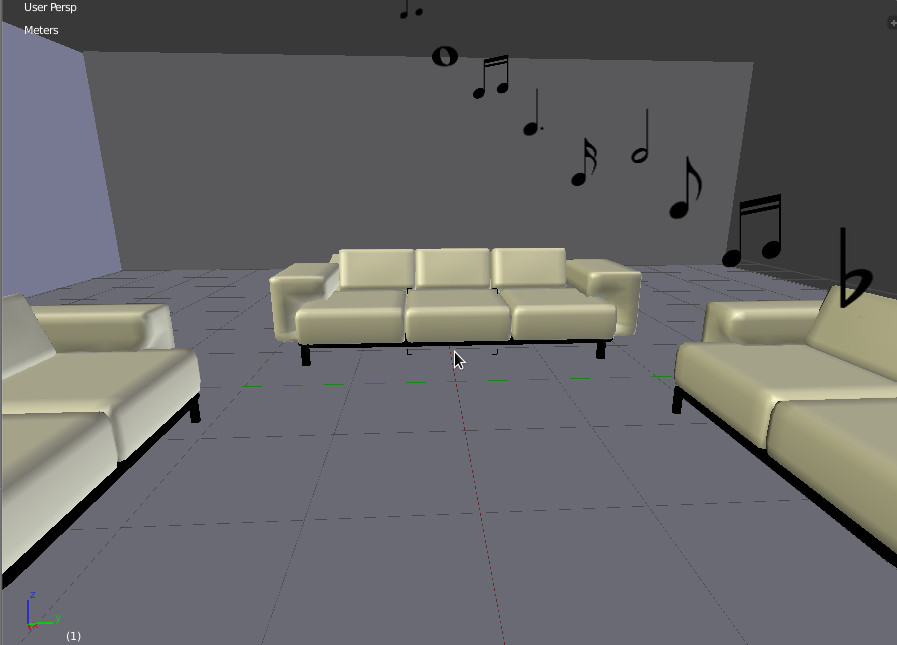
\includegraphics[width=90mm]{images/GD_basic.jpg}
\caption{Room with one object generating sound}
\label{sensorymockup1}
\end{figure}

\begin{figure}[H]
\centering
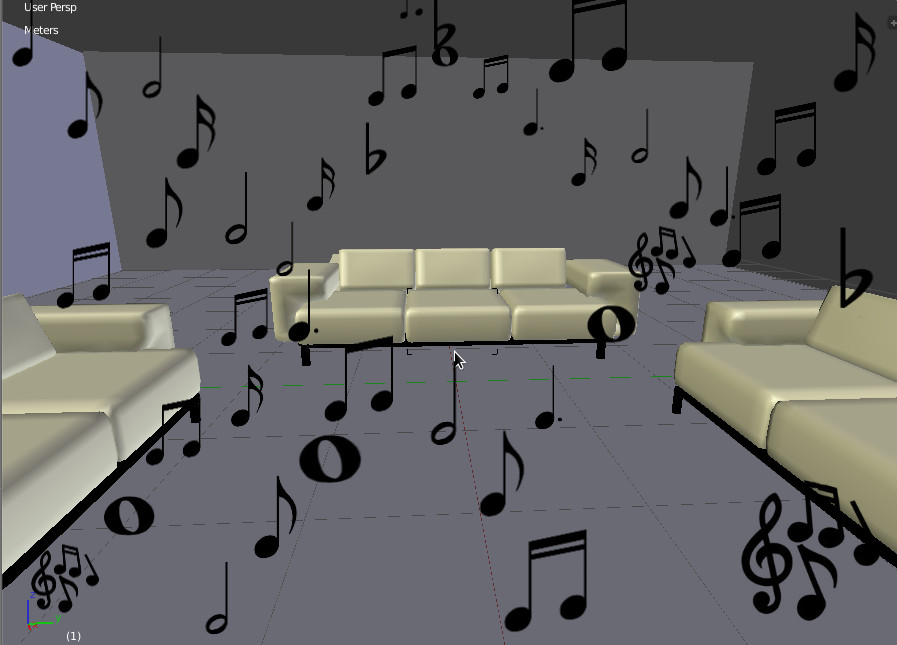
\includegraphics[width=90mm]{images/GD_moresound.jpg}
\caption{Effects of multiple objects creating sound}
\label{sensorymockup2}
\end{figure}

\begin{figure}[H]
\centering
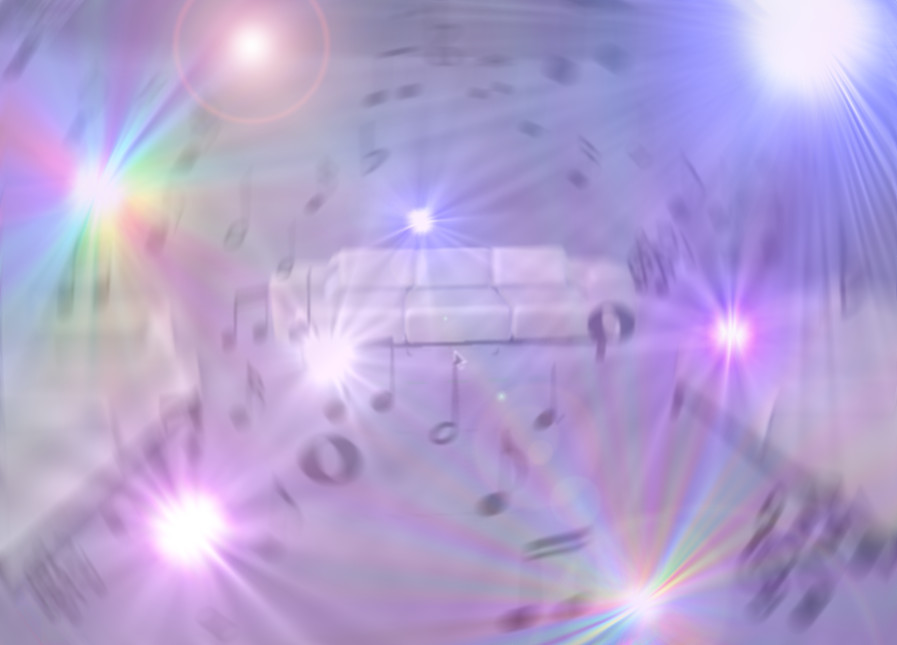
\includegraphics[width=90mm]{images/GD_overload.jpg}
\caption{Sensory overload. Lights have become brighter and environment is harder to see. Gaussian filter applied}
\label{sensoryoverloadmockup}
\end{figure}

2 of the 3 people interviewed specified that found the below image uncomfortable to view and was quite accurate. This demonstrates again that a sensory overload differs for each individual and indicates more should be consulted as 3 is a small sample. However, the projects core aim is to raise awareness of these problems rather than attempting to give an identical experience of having autism and thus this approach will be used unless feedback in the formative evaluation indicates changes are required. 

Sensory overloads will affect and be affected by the players contentment. If the player does not move away from troublesome objects quick enough, contentment will drop, which, if not addressed quick enough can lead to a meltdown. In addition, if contentment is low sensory overloads will occur quicker. 

\subsubsection{Special interests}
'Special interests' were chosen as a way to alleviate some of the difficulties within the environment and as a means to replenish energy or contentment. When engaging with a special interest, troublesome sounds will be reduced and if experiencing a sensory overload or meltdown the effects will subsidise. The special interest selected will be a Dinosaur toy which the user can interact with.

\subsubsection{Information processing delay}
Information processing delay was highlighted in interviews by a teacher as one of the main causes of meltdowns in school. When the user clicks on an object to interact or is expected to give a response, actions will be made harder to select by moving around. If the character has lower contentment the selections will move even quicker which should result in a greater delay from the player. Such delays could affect responses from other characters in the game. 

\subsection{Tool selection}
It was decided to use a game engine to allow time and focus to be directed onto the higher level concepts. Suitable game engine candidates were identified by looking at those highly rated on gamedev.net (extensive online resource for game developers), whilst taking some previous knowledge into account. Blender will be used as the modelling tool as it is freely available, powerful and well supported with lots of tutorials and documentation.

\subsubsection{Game engines}

** Put this in a table

\textbf{Unity}\\
Unity is one of the most popular game engines available with good support for models. Unfortunately the licence costs 1500 and the free version comes with limitations.

Advantages: popular game engine to use. Quick development with scripting. Phone app support.\\
Disadvantages: Interface heavy, limited to just scripting, costs, good computer required to run it efficiently.

\textbf{JMonkey}\\
JMonkey is a java 3d game engine that has been in development around for a few years. It has an extremely active and helpful community, allows complete customisation and holds little limitation being open source.

Advantages: Provides development environment with scene graph. Active community where you often get responses from developers themselves. Java is quick to develop in. Support for online use and phone apps. \\
Disadvantages: Java is not seen as the preferred language for graphics or games.

\textbf{Panda3D}\\
Originally created by Disney, Panda3D is an engine which can be used via python or C++ although support is mostly for python.

Advantages: Quick to develop for with a choice in language. Good community with lots of tools.\\
Disadvantages: No phone app and limited online support. Lack of documentation. 

\textbf{Ogre3D}\\
Ogre3d is primarily a graphics rendering engine and but it does have additional plugins such as 'physics' or drawing interfaces.

Advantages: Lots of modules and plugins. Powerful and used commercially. Active support community.\\
Disadvantages: Longer development process. Lack of tools such as a scene graph. No support for putting online.\\

JMonkey was chosen for its active community, development environment, because its programmed in Java and open-source. Although Java is not seen as the programming language of choice for graphics it allows quicker development than C++ counterparts. Unity allows very quick development with great results but the pro version would be required for some features, which is very expensive. As JMonkey is in Java it can be easily transferred to both an online game and an Android app which increases accessibility. Although an Android app may not be possible during the project timeline, converting the game to online should be straightforward. Finally there were no foreseen limitations with using JMonkey.

\subsubsection{Modelling tools}
For modelling there several options:
\begin{itemize}
\item Maya
\item 3DSMax
\item Blender
\item Sketchup
\end{itemize}

Blender was the primary 3D modelling tool of choice as it is free, open source, widely used for various game developers and professionals and the tool JMonkey is most built to accommodate.


\subsection{Character}
The character the user will play as. What difficulties they have/ what age they are.


\chapter{Prototype}

\section{Implementation}
The program structure was built from scratch using JMonkey. The scene contains a model of a house which was produced in sketch-up and contains two bedrooms, a kitchen and a living room all on one door). More detailed furniture models were created in blender and some (such as the character model) were taken from free online repositories. Particle emitters were added to models that were a source of sound in order to visually represent the sound disturbances reported by those with autism(the more objects emitting sound that the player is near, the harder the environment will become to view and as such it should intuitively prompt them to move away).

\section{Gameplay}
The player moves around and explores a realistic home environment. They are able to interact with the environment, such as turning of lights, opening and closing doors. Their well-being is monitored at all times by a contentment gauge visible on screen. The players goal is to interact with the environment, and later perform specific tasks, while
maintaining contentment at a high level. If contentment drops, this is represented by the gauge graphic and when it reaches zero, the player experiences a meltdown and restarts. When being affected by unpleasant sensory inputs
such as light or sound there is an introduction of visual flters on screen which are uncomfortable to view and inhibit accurate navigation of the environment and task completion. The player can perform various activities to increase contentment again.

\subsection{Game modes}

\subsubsection*{Task mode}
In the task mode, the user is required to navigate around the environment
whilst experiencing some of the sensory obstacles in order to complete tasks.
In essence, this is the game or story mode of the program.

The program structure is designed to allow flexibility when giving the
user tasks to complete in the environment. "Tasks" are java classes which can be dropped into the system and loaded. These classes can define custom actions on objects which may only be applicable when the task is active, e.g,
get a drink, get dressed, ask Mum for help. Task classes must also set the conditions for completion such as player is holding a drink, is dressed, spoke to mum and on completion the next task is selected and displayed to the
user. One of the benefits of this comes with testing as specific tasks can be selected and it doesnt require going through a series of events to trigger the tasks that need to be checked or needing to comment out large portions of
code.

\subsubsection*{Exploration mode}
In the exploration mode the user can navigate and explore the environment without the worry of the contentment bar reaching zero or meltdowns although sensory disturbances still occur.

\subsection{Autism aspects}

\subsubsection{Representing sensory overloads and meltdowns}
The three sensory problems currently implemented are sensitivity to sound, light and tactile. The proximity and amount of objects around the player will firstly affect the sensory health. When this falls below a specified threshold
the first level of a sensory overload occurs and the impact of surrounding objects become more prominent, lights becoming brighter for example. If the player does not move away, the second level is reached in which visual effects
worsen making it harder to see, a representative of a sensory overload. When the first level is reached, the contentment bar is slowly reduced and when the second level is reached and a sensory overload occurs the reduction is quicker, reflecting the exponential impact of unpleasant sensory stimulus
over time.

The sensory system both effects and is affected by the contentment bar which is the equivalent of a players "health" or well-being. Interviews showed that if someone with autism is feeling particularly drained from their day or
awakens feeling particularly anxious their tolerance to their surroundings is lower and hence when contentment is lower, a sensory overload is more likely to occur. Translating the information from interviews and readings to
implementation proved challenging because of the amount of differing information. The specific triggers do require work and adjustment, for example having only certain types lighting causing problems as currently all of them
are. Sound is currently represented by visual sound waves emitting from objects and these need to be made bigger and more dense so that the more sound-emitting objects around, the more disturbances occur and the harder
it is to interact with surroundings. A final improvement is for contentment to slowly increase if not around any objects causing sensory problems and if not around people.

\begin{figure}[H]
\centering
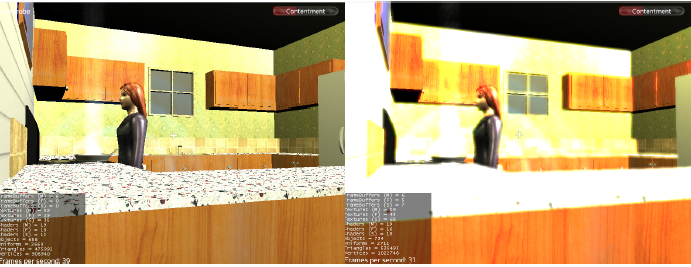
\includegraphics[width=110mm]{images/old_sensoryeffects.png}
\caption{Light sensory effects: representing the impact of disliked bright
light on the visual experience of a child with autism(right)}
\label{old_sensoryeffects}
\end{figure}

\subsubsection{Effects on contentment}
Contentment of the player reduces when experiencing sensory overload effects and will stop reducing after a period of time if the player moves away from them. There are other specific actions within the game that will also cause the
contentment to reduce such as getting dressed(to represent tactile sensitivity) or being told off by the parent. Currently the contentment can replenish if the player engages with special interests which are represented in-game as playing with the dinosaur. More will be implemented later to reflect some of the other experiences that those with autism find soothing.

\subsubsection{Other features}
\textbf{Information processing delay}: The delay in information processing exhibited by someone with Autism is demonstrated by creating a options which represent in-game choices which constantly rotate, making it harder
to read, choose and also select a response. The speed in which this occurs is dependent on the contentment level so that the less content the character is, the harder it becomes to make a choice as they rotate faster. \\

\textbf{Description box}: Users can click on certain objects and obtain information in the form of pop up boxes on certain items that may cause problems or be of interest to someone with autism. I.e explaining that information on
TV may be taken literally and a child may thus expect a toy to react in the same way as advertised or may not be able to identify that what is seen on TV is not real. This adds an extra layer to the system allowing a person
to visually walk around an environment and learn about Autism which may alone be more effective and engaging than reading a textbook on the topic. \\

\textbf{Special/repetitive interests}: Interactions with favourite objects such as a toy dinosaur cause contentment to slowly increase whilst reducing any sensory problems, reflecting one known real-world function of such repetitive interests.

\subsection{Overcoming challenges}
At the start of the project significant amounts of time were spent trying to import rather than create models. It was a tedious task because small changes to the models required the whole house scene to be remade in JMonkey or
time had to be spent on editing models better work with JMonkeys import system. It also became evident from using Blender that it has a very steep learning curve and is a tool which can take some considerable time to master.
However, in the last two months of the game development process, these obstacles have been largely overcome. Experience acquired, coupled with updates in February to the JMonkey import system, made it easier and less
time consuming to acquire, create, change and import models. The whole scene was no longer required to be rebuilt allowing time to be better spent. Moreover, the update allowed direct use of google sketchup, a 3D modelling
tool which is easier and quicker to use than Blender (although it produces less quality assets) and offers a wealth of free models in the online repository, most of which are home components such as furniture.

Overall, JMonkey has proven to be a good choice. No additional limitations have been found and development was quick once a solution was found to the model import pipeline. The modularity offered by Java allows
further extensions to be created with ease without needing to change a large portion of the program structure. Finally, being able to combine sketchup and Blender has been a great help and with practice, asset creation should
continue to speed up.

\subsection{Technical}
More technical information of the programming. Class and system diagrams.

- Explanation of missions interface \\
- Scenes\\
- object states\\
- player class\\
- gui\\
- action manager\\
- Class diagrams\\


\section{Evaluation}
The current version of the simulator has been evaluated in two settings. The first was the presentation of the simulator to the LAERLab group(see below). The second was a questionnaire sent to some parents/family members of children with autism and adults with autism.

TODO: More details information on the evaluations, specifically the LAER one.

\subsection{Expert feedback}
The LAER group consists of students and academics with an interest in the field of accessible and educational technology design. A focus group of 10 members provided comments and feedback. A short video demo was presented and narrated, showing exploration of the environment and then one task being completed (which was to obtain a drink from the kitchen) including demos of sensory overload effects, meltdown and information processing delay concepts.

\subsection{User feedback}
A video was sent out with verbal instructions and descriptions along with a questionnaire which was filled out by 1 family member and 3 parents of children with autism as well as and 3 people with autism. It contained both qualitative and quantitative questions.

\begin{table}
\caption{Questionnaire results. Participants responded giving an answer between 1 and 5. 5 being the highest rating}
\begin{tabular}{| p{9cm} | c c c c c |}
\hline
\textbf{Question} & 1 & 2 & 3 & 4 & 5 \\
\hline
How likely would you be to play the simulator? & 0 & 0 & 1 & 2 & 4 \\
\hline
How much do you think playing the simulator could help you understand the behaviour of a child with autism better? & 0 & 0 & 0 & 2 & 5 \\
\hline
How much did you like the visual effects? & 0 & 0 & 1 & 3 & 3 \\
\hline
How much did you like the graphics? & 0 & 0 & 2 & 2 & 3 \\ 
\hline
\end{tabular}
\end{table}

The qualitative questions asked were:
\begin{enumerate}
\item Who would you think the simulator would be useful for?
\item How accurate do feel the representation of a sensory overload is? Please include any additional comments.
\item Do you have any other scenarios, examples or information(that could go in description boxes for example) that could be offered that you think may be useful for others?
\end{enumerate}

Overall feedback in relation to qualitative question 3 was that the sensory overload representation was good but "more effort in depicting the pain felt from sound would be good". 

** put more of the responses from the simulator questionnaire in here.

\section{Improvements planned}
Following constructive feedback from these sources, the following amendments to the simulator have been prioritised:

\begin{enumerate}
\item Some viewers with autism commented they found it difficult to watch as it was causing them to have a sensory overload. Thus, one improvement is to allow certain effects/components to be turned on or off.
\item Remove pop-up description boxes which users felt interrupted the simulation and instead represent this information in a side-bar.
\item Improve game-play controls which are currently too sensitive and make viewing difficult.
\item Adjust threshold for a meltdown occurring as these are happening too quickly.
\item Certain objects should present more sensory problems than others i.e fire alarm causing a quicker reduction in contentment than the noise from the TV. Overall, comments in relation to the sensory overload effects were very positive.
\end{enumerate}

Interviews need to be further conducted with parents, teachers and carers to and more scenarios with which they commonly experience difficulty. Such information can be used to create a storyboard of scenarios and tasks. As
well as gathering information from individual interviews, the simulator will also be presented at a workshop for a charity to an audience of carers of children with autism and other disabilities. This could be given in the form of a visual demo and/or allowing them to play.

\chapter{First version: Latest work}
The following includes the latest work carried out on the simulator over the semester which includes planning, changes and implementation. 

The first version underwent more substantial changes than previously planned. Large parts of the system were rewritten and improved upon such as the GUI and sensory manager. The benefits resulted in simplification of use at the higher level (such as implementing storyboards) and a better representation of the causes of sensory overloads.

Selecting actions to interact with objects is now less intrusive. Prior a menu would pop up and prompt the user to make a selection with their mouse which will now only happen if there are multiple options. With the removal of description boxes, thoughts are now displayed at the bottom of the screen when to user is looking at a specific object.

Performance issues which were not previously too severe now required direct attention. The game requires a frame rate of 30fps(frame per second) or above in order to be fluent and played without lag. Scenes are required to have a maximum of 100k vertices(from models) with an average of 10-50k. Each pointlight(which is a light the user can turn on/off) used requires the scene to be rendered again and so the number of vertices double with each point light used. Thus, even when keeping within the limits, the amount of lights being used in the game was pushing it to well over a million and the frame frequently dropped below the desired threshold. This was occurring on a computer with a decent processor and graphics card, thus playing on a low-powered machine would not be a good experience.  

Having originally taken a large amount of models from other websites and using programs such as sketchup to aid quicker development, these were found to be inefficient at runtime. Efforts therefore were spent on re-learning the details of blender and what is required to make lightweight game models. 

Where previously the entire house modelled and then imported, the solution to the above problem was to split the house into individual rooms/scenes. When the user then clicks a door, the required scene is loaded very quickly. This approach allows for inclusion of more detailed models within each scene as each scene is only a small room. The problems to performance caused by point lights is then reduced as it is only rendering a single room again, not the entire house. 

Further benefits from compartmentalising the house into rooms arose for dealing with the model pipeline. It became much easier to create individual models and link them into the scene, so if the model needed to be edited it could be without requiring the pain of reimporting and fixing textures or materials. 

The result of the restructure meant the FPS improved tenfold, from an average of 30fps to 200-400fps. If any objects were found to be creating problems from being too detailed or not textures properly, they could be removed without impacting on the rest of the scene.

\section{Storyboards}
Following the prototype which had little story or goals a more in-depth story and set of tasks were created. The user will play as an example "Day in the life of a child with autism". This will be split up into several "Missions"(tasks).

\subsection*{Mission 1: Complete morning routine}
Complete your morning routine in the designated time(the more out of time, the more contentment drops). Player starts in the bedroom which is a designated safe place/sensory room. 

Routine to complete: eat breakfast, brush teeth, get dressed.

\textbf{Game points}
\begin{enumerate}
\item User progresses to the kitchen for breakfast. Possibly use a particle emitter to make lots of ‘germs’ appear in the kitchen.
\item After breakfast the user must go to the bathroom and brush teeth which reduces contentment due to bristles harsh texture. Noise from the toilet scares and prompts the the user to run out of bathroom into the hallway.
\item The lamp in the hallway however has now been turned on and the hallway looks different, the light causes discomfort. The character freezes and the player is unable to move forward but can move backwards. The user can turn the lamp off at the plug but at this point may not be aware of this. If a meltdown occurs, start back in the bedroom with a message that you can turn the lamp off at the plug. When the user returns from a meltdown contentment will not be at its maximum.
\item User clicks wardrobe to get dressed, information displays explaining that certain clothing can feel extremely uncomfortable for someone with autism and can be compared to sandpaper.
\item Morning ends in the bedroom with player not wanting to leave (the plug to the lamp is away from the bedroom so the player has to pass lamp to turn it off) and trying to play/recuperate. Parent then comes in and says “Cmon, we need to go out!”.
\item Child has a meltdown, thoughts flood the screen with fears and anxieties. Where are we going? Are we taking the car? When will I be back? Stomach hurts, stomach hurts - words become even more jumbled. They weren't warned and thought they could replenish energy levels in their room, the change means the rest of the day could be faced with countless unprepared fears.
\end{enumerate}

\subsection*{Mission 2: Afternoon, find out the cause of stomach pain}
Mission is to find out why the characters stomach may be hurting which also gives the user a chance to explore. Contentment slowly drops until the solution is found. Reasons for the pain could be:

\begin{itemize}
\item Hunger/Thirsty
\item Upset stomach or cramps
\item Toilet?
\end{itemize}

The user will be expected to attempt all of the above(the final one the user finds will always be the cause). During the above the door bell will unexpectedly ring and a new character will enter, the Mum's friend. The friend was meant to be meeting you both out but due to the earlier meltdown has come to the house instead. Mum tried to explain in advance but words weren't making sense. The person looks like a stranger and can't be recognised and contentment reduces(touch sensitivity occurring from this stranger?). 

\subsection*{Mission 3: Evening, get to bed}
Mission pops up that it is time to go to bed but mum stops you and says you can continue playing. Mum then approaches after an unknown amount of time and informs you to go to bed. Meltdown occurs as it's not the exact time and the characters bedtime routine has been broken.

\section{House design}
Following a need to compartmentalise the previous house environment as a solution to performance issues, a new and more structured plan of the house was created. The game description column of the table is information the user will see when they interact with the object and will be displayed as "thoughts":

\begin{table}[H]
    \begin{tabular}{| p{2cm} | p{2cm} | p{3cm} | p{3cm} | p{4cm} |}
    \hline
    Room & Object & Action & Game description & Effects                                                                  \\
    \hline
    \hline
     Bedroom & Dinosaur & Play: Increases contentment by playing with it & People with autism have special interests. These special interests help with xyz &                   \\
    \hline
    & Touchside lamp & On/off: slowly adjust the light so it does not turn off rapidly. Contentment goes up when light turned off slowly & & If the light goes off too quickly, contentment increases slightly but then rapidly declines. Room looks strange/scary as eyes not yet adjusted    \\
    \hline
    & Collections of items & & Explains that children with autism have an obsession/need to complete collections &  \\
    \hline
    & Wardrobe & Get dressed & Explanation that clothes can be compared to feeling sandpaper & Contentment reduces  \\
    \hline
   & Spinny object & & & All noise blurs out. Contentment increases \\
    \hline 
    Upstairs hallway & Fluorescent light & Turn on/off. Same effect as bedside lamp & Explanation about fluorescent lights. Effects are like ten camera flashes in your eyes & Lights flicker and cause a 'high' effect on sensory system. Disorientation if exposed too long. \\
    \hline
    & Mirror & "Look into" & I don't recognise this person. Not normal having yourself peering back at you & Causes dizzy/disorientation because it is an odd image to see. \\
    \hline
    & Wallpaper & & & Make wallpaper material move and cause dizziness/sensory effects. \\
    \hline
        Downstairs hallway & Flowers & & & They can either smell good or bad. \\
    \hline
    & Door bell & Automated: on/off & Nicer sound could prompt the user to play with it. Can cause anxiety as doorbell may mean unwanted people in safe space & If player rings it is fine. If another person, causes problems.
    \\
    \hline
    \end{tabular}
\end{table}

\begin{table}[H]
    \begin{tabular}{| p{2cm} | p{2cm} | p{3cm} | p{3cm} | p{4cm} | }
    \hline
    Room & Object & Action & Game Description & Effects                                                                  \\
    \hline
    \hline
        Kitchen & Washing machine & Turn on/off & Could become transfixed with spinning nature & Noisy, need to move away. \\
    \hline
    & Kitchen sides & & Particle emitters to show germs/smells & Reduces contentment \\
    \hline
    & Frying pan & & & Sounds, smells, contentment reduction \\
    \hline
    Living room & TV & Turn on/off & Description indicating that child may think items on TV are identical to what they will get & TV being too loud may hurt. \\
    \hline
    & Hoover & & Description indicating that the noise from Hoovers can be painful & Sensory problems when turned on \\
    \hline
    Bathroom & Bath & Empty bath & & Horrible/scary noises. \\
    \hline
    & Tooth brush & & & Brushing teeth causes contentment to reduce. \\
    \hline
    \end{tabular}
\end{table}


\section{System changes}
** TODO: Add diagrams and more in-depth information/diagrams. Quite a few of the technical system changes were made several months ago, so need to create diagrams of initial set ups and current to give a better comparison and details in final thesis.

\subsection{Rewrite of scenes}
Most the the effort in the last few weeks of the semester were spend on re-writing the scene manager and remodelling the house. 

\begin{figure}[H]
\centering
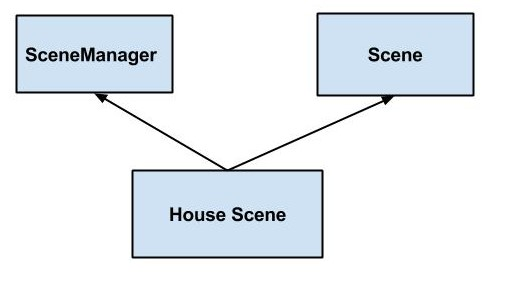
\includegraphics[width=90mm]{images/scenemanager.jpg}
\caption{Overview of the previous house that was used}
\label{old_house}
\end{figure}

SceneManager contains useful tools for the creation, deletion and changing of scenes. The "HomeScene" extends this and contains objects which are all instances of Scene and represent the individual rooms. By extending the SceneManager the HomeScene can listen to events occurring in the game and specify custom ones that are unique for that collection of scenes(or rooms), for example it can specify that doors require changing and loading of different rooms. 

\subsubsection{House implementation}
In addition to remodelling parts of the house a bathroom was created and added along with new actions such as being able to flush the toilet(with sounds to accompany this). Now being able to handle individual objects in rooms allows for easy addition animation, the clock's hands in the room move and will indicate the time of day. Below gives some screen shots of the new environment and it's accompanying frame-rates. 

\begin{figure}[H]
\centering
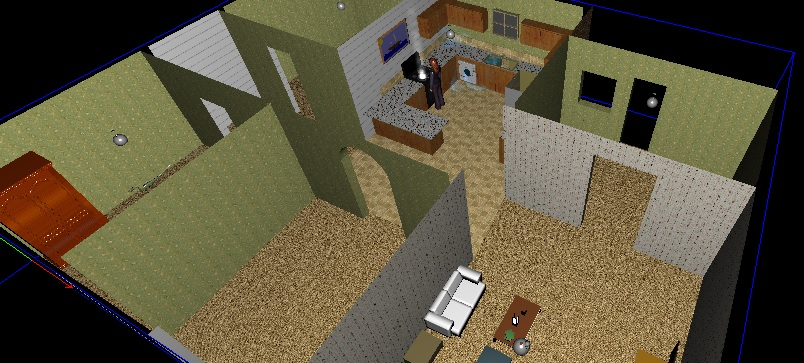
\includegraphics[width=90mm]{images/old_fullhouse.jpg}
\caption{Overview of the previous house that was used}
\label{old_house}
\end{figure}

\begin{figure}[H]
\centering
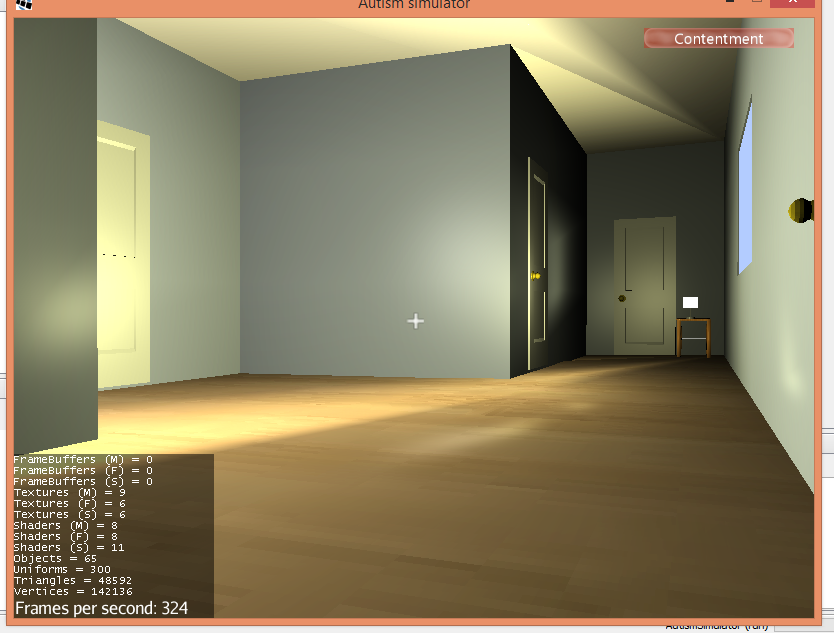
\includegraphics[width=90mm]{images/new_hallway1.png}
\caption{Overview of the previous house that was used}
\label{old_house}
\end{figure}

\begin{figure}[H]
\centering
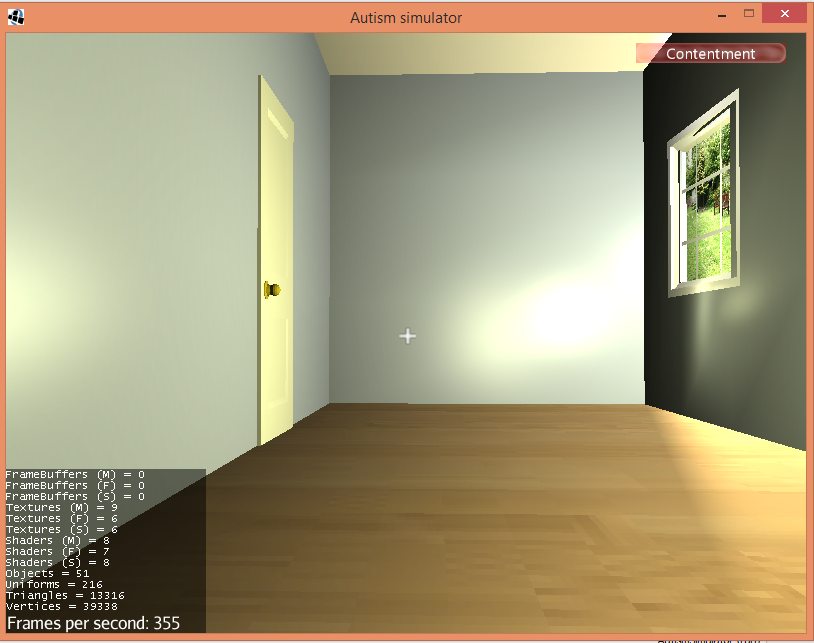
\includegraphics[width=90mm]{images/new_hallway2.png}
\caption{Overview of the previous house that was used}
\label{old_house}
\end{figure}

\begin{figure}[H]
\centering
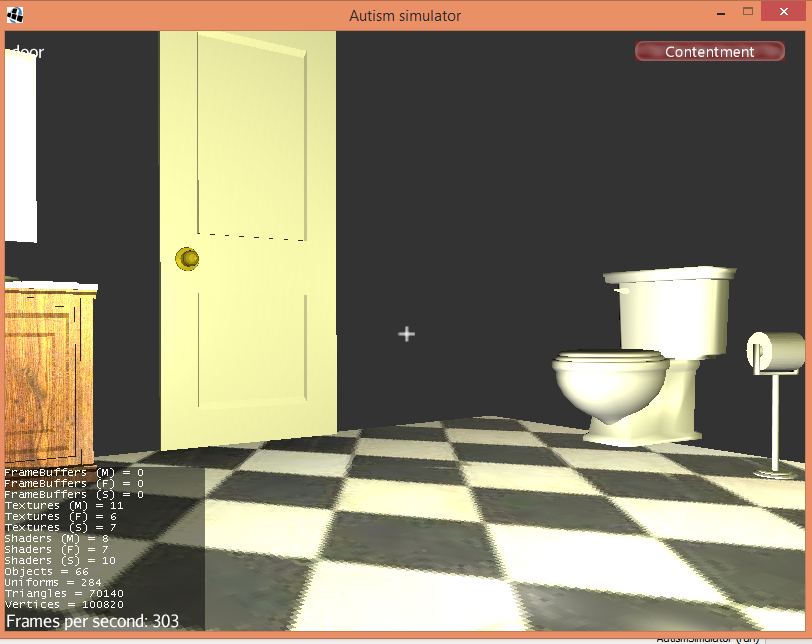
\includegraphics[width=90mm]{images/new_bathroom.png}
\caption{Overview of the previous house that was used}
\label{old_house}
\end{figure}

\begin{figure}[H]
\centering
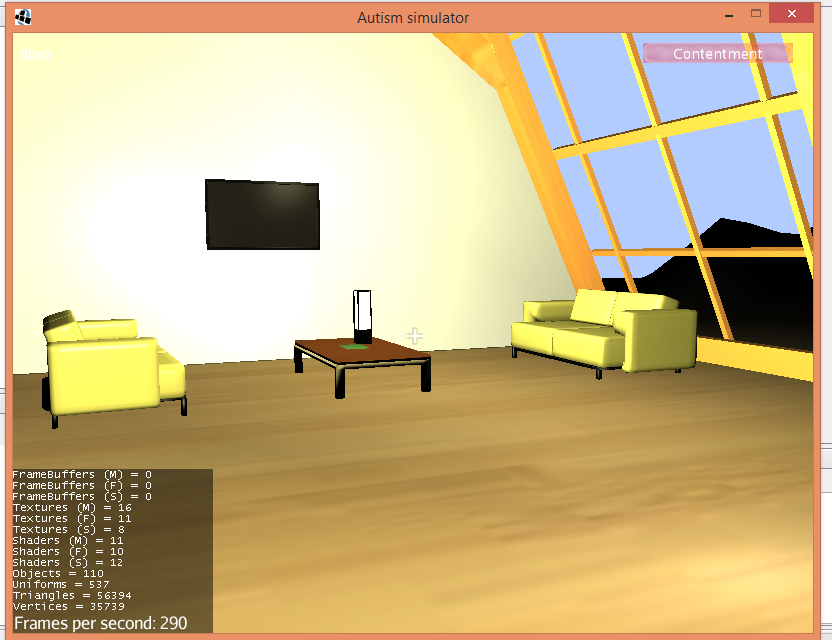
\includegraphics[width=90mm]{images/new_livingroom.png}
\caption{Overview of the previous house that was used}
\label{old_house}
\end{figure}

\subsection{Game state manager}

As the size of the system grew, one of the most important changes was the addition of a game state manager, enabling universal control and monitoring of the overall system. 

The user can now change between "Explore mode"(the user has no tasks and can simply look around the environment) and "Mission mode"(given the tasks or story) without having to restart the simulator. From this came the addition of the start and help screen and ability for the user to pause the game.  

The rest of the system can now request useful information from the GSM such as which mission is currently being run, which scene the player is currently in and what the state of the GUI is (if actions are being displayed, if the user is required to select an option). If the GUI needs to display information(such as selecting actions) it will notify the game state manager which will halt processes that may interfere. Having a central control made other parts of the simulator easier to develop and reuse since each part of the system only needs to worry about which state it is in rather than checking multiple conditions.

\subsection{Sensory System improvements}
Following the feedback on sensory overloads, improvements were required in how sensory overloads occurred rather than what was happening when they did. Previously, objects which could affect the sensory system were put into a Hashable which were then periodically checked for the distance to the player and if in proximity, would affect the sensory system depending on how far the object is. However, all objects would affect the user by the same weight and the effect on contentment would change depending on what threshold of objects were reached (i.e if 2 were in proximity the health reduction would be low, if more than two the reduction would be greater). Filters to mirror sensory overloads would then be applied depending on this level.

\begin{figure}[H]
\centering
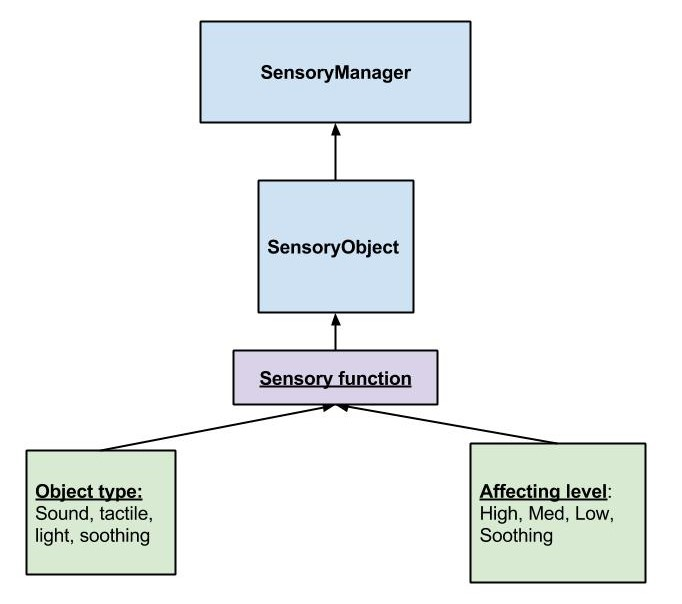
\includegraphics[width=90mm]{images/sensoryobjects.jpg}
\caption{Diagram showing implementation of sensory system}
\label{sensorysystem}
\end{figure}

The new implementation attempts to create a better less fragmented model of how objects affect the player and cause sensory overloads/meltdowns. This approach is more scalable and enables a flexible means to experiment by simply changing parameters, thus helping to address previous issues of meltdowns occurring too quickly.

Each sensory object is given two properties (from the green boxes above) and from this a sensory function is applied and a weight for each object is calculated. The sensory function is simply an exponential: the higher the affecting level the higher the weight returned and if the object is set as a 'soothing object' a negative value will return instead. 

The sensory manager then takes all the weights of the objects that are in proximity and sums them, taking the log of this. If the log is negative there are no objects and contentment replenishes. The result of the summation is then taken away from the players contentment. 

Sounds were the final addition to the simulator. When acting on the toilet it now flushes and the alarm clock in the room rings. Sounds create a more immersive environment and an additional layer for creating sensory overloads(i.e making objects more high-pitched). 

\chapter{Formative evaluation}
The formative evaluation will be carried out with 5 participants and will be predominantly testing usability, checking that accompanying materials such as help-guides and game controls.

\chapter{Summative evaluation}

\chapter{Conclusion}

\chapter{Plan and future work}

Additions to simulator prioritised as required for the formative evaluation:

\begin{enumerate}
\item Change start screen to have an image behind it with a more informative help screen.
\item Recording of sounds: Door bell, TV noise.
\item Spinning soothing object in bedroom.
\item GUI changes: Make thoughts more readable as they can be quite difficult with certain backgrounds.
\item Completion of storyboard implementation: morning routine is complete as is the afternoon(except the doorbell and introduction of another character) but needs final touches.
\item Tooltip: As the process of selecting actions was changed it is not obvious what will happen when the user interacts with other objects or what room they will walk into when clicking on a door. A tool-tip would be an easy addition that would not interfere with play.
\end{enumerate}

\begin{table}[H]
\begin{tabular}{| p{8cm} | p{4cm} | }
\hline
Task & Deadline \\
\hline
Complete plan for formative evaluation & January 24th \\
\hline
Finishing additions and improvements to simulator & February 3rd \\
\hline
Start formative evaluation & February 4th \\
\hline
Finish formative evaluation & February 6th \\
\hline
Improvements to simulator based on feedback & February 17th \\
\hline
All sections of dissertation complete(except summative evaluation) & February 17th \\
\hline
Summative evaluation & February 21st(end of ILW) \\
\hline
Completion of dissertation writing & March 6th \\
\hline
\end{tabular}
\end{table}


\begin{thebibliography}{9}

\bibitem{increasingprevalence}
Johnny L. Matson, Alison M. Kozlowski
The increasing prevalence of autism spectrum disorders. Research in Autism Spectrum Disorders(2011)

\bibitem{nas}
National autistic society. www.autism.org.uk

\bibitem{statsandfacts}
Ambitious about autism. www.ambitiousaboutautism

\bibitem{nasschool}
Make school make sense. Autism and education: the reality for families today. National Autistic Society, 

\bibitem{autismmisconception}
Autism misconceptions. NHS

\bibitem{olgab}
Sensory Perceptual Issues in Autism and Aspergers syndrome(2003). Bogdeshina, O

\bibitem{fears}
Unusual fears in children with autism(2012). Susan Dickerson Mayes, Susan L. Calhound, Richa Aggarwal, Courtner Baker, Santosh Mathapati, Sarah Molitoris, Rebeccas D. Mayes.

\bibitem{temperament}
Sensory correlates of difficult temperament characteristics in preschool children with autism(2012). I-Ching Chaung, Mei-Hui Tseng, Lu Lu, Jeng-Yi Shieh

\bibitem{bayes}
When the world becomes 'too real': a Bayesian explanation of autistic perception(2012). Elizabeth Pellicano and David Blurr.

\bibitem{williams1996}
Autism: An inside-out approach(1996). Williams, D

\bibitem{williams1994}
Somebody Somewhere: Breaking Free from the World of Autism(1994). Williams, D.

\bibitem{williams1992}
Nobody no-where(1992). Williams, D

\bibitem{sensory_leisure}
Sensory processing abilities and their relation to participation in leisure activities among children with high-functioning autism spectrum disorder. Hochhauser, M. Engel-Yeger, B.

\bibitem{sensory_toddlers}
Parent Reports of Sensory Symptoms in Toddlers with Autism and Those with Other Developmental Disorders. Sally J. Rogers, Susan Hepburn, Elizabeth Wehner

\bibitem{sensory_children}
Describing the sensory abnormalities of children and adults with autism(2007). Susan R. Leekam. Carmen Nieto. Sarah J. Libby. Lorna wing. Judith gould. 

\bibitem{sensory_perceptual}
Sensory integration and the perceptual experience of persons with autism(2006). Grace Iarocci. John McDonald.

\bibitem{rss_cognitive}
Restricted and Repetitive Behaviours, Sensory Processing and Cognitive Style in Children with Autism Spectrum Disorders(2009). Yu-Han Chen, Jacqui Rodgers, Helen McConachie.

\bibitem{rrsyouth}
Restricted and repetitive behaviours and psychiatric symptoms in youth with autism spectrum disorders(2013) Elizabeth A. Stratic, Luc Lecavlier.

\bibitem{rrs_sensory}
Is there a relationship between restricted, repetitive, sterotyped behaviours and interests and abnormal sensory response in children with autism spectrum disorders?(2008). Robin L. Gabriels, John A. Agnew, Lucy Jane Miller, Jane Gralla, Juliet P. Dinkins, Elizabeth Hooks.

\bibitem{aspieway}
"It’s like you are just a spectator in this thing": Experiencing social life the 'aspie' way(2008). Sara Ryan, Ulla Raisanen

\bibitem{dd}
Disability awareness: Beyond the day: http://www.serviceandinclusion.org/index.php?page=simulations. Danielle Dreilinger

\end{thebibliography}

\end{document}